\begin{enumerate}[label=\thechapter.\arabic*,ref=\thechapter.\theenumi]

\item Consider a unity-gain negative feedback system consisting of the plant $G\brak{s}$  and a proportional-integral controller. Let the proportional gain and integral
gain be 3 and 1, respectively. For a unit step reference input, the final values of the
controller output and the plant output, respectively, are
\begin{align}
    G\brak{s} = \frac{1}{\brak{s-1}} \notag
\end{align}\hfill (GATE EE 2023)\\
\solution 
\iffalse
\let\negmedspace\undefined
\let\negthickspace\undefined
\documentclass[journal,12pt,twocolumn]{IEEEtran}
\usepackage{cite}
\usepackage{amsmath,amssymb,amsfonts,amsthm}
\usepackage{algorithmic}
\usepackage{graphicx}
\usepackage{textcomp}
\usepackage{xcolor}
\usepackage{txfonts}
\usepackage{listings}
\usepackage{enumitem}
\usepackage{mathtools}
\usepackage{gensymb}
\usepackage{comment}
\usepackage[breaklinks=true]{adjustbox}
\usepackage{tkz-euclide} 
\usepackage{listings}
\usepackage{gvv}                                        
\def\inputGnumericTable{}                                 
\usepackage[latin1]{inputenc}                                
\usepackage{color}                                            
\usepackage{array}                                            
\usepackage{longtable}                                       
\usepackage{calc}                                             
\usepackage{multirow}                                         
\usepackage{hhline}                                           
\usepackage{ifthen}                                           
\usepackage{lscape}

\newtheorem{theorem}{Theorem}[section]
\newtheorem{problem}{Problem}
\newtheorem{proposition}{Proposition}[section]
\newtheorem{lemma}{Lemma}[section]
\newtheorem{corollary}[theorem]{Corollary}
\newtheorem{example}{Example}[section]
\newtheorem{definition}[problem]{Definition}
\newcommand{\BEQA}{\begin{eqnarray}}
\newcommand{\EEQA}{\end{eqnarray}}
\newcommand{\define}{\stackrel{\triangle}{=}}
\theoremstyle{remark}
\newtheorem{rem}{Remark}

\begin{document}
\bibliographystyle{IEEEtran}

\vspace{3cm}

\title{}
\author{EE23BTECH11024 - G.Karthik Yadav$^{*}$
}
\maketitle
\newpage
\bigskip

\section*{GATE 2023 EC 41}
\noindent 1. \hspace{2pt} A Closed loop systen is shown in the figure where $k>0$ and $\alpha>0$ .\\
The Steady State error due to a ramp input $\brak{R\brak{s} = \alpha s^{-2}}$ is given by \hfill{(GATE 2023 EC 41)}

\begin{figure}[ht]
\centering
    \includegraphics[width=1.0\linewidth]{2023/EC/41/figs/question.png}
    \label{fig: 23.EC.41.24.1}
\end{figure}

\begin{enumerate}
\item $\frac{2\alpha}{k}$
\item $\frac{\alpha}{k}$
\item $\frac{\alpha}{2k}$
\item $\frac{\alpha}{4k}$
\end{enumerate}

\solution\\
\fi
\begin{table}[ht]
\setlength{\arrayrulewidth}{0.3mm}
\setlength{\tabcolsep}{15pt}
\renewcommand{\arraystretch}{1.5}



\begin{tabular}{ |p{1cm}|p{3cm}|p{1cm}| }
\hline
Symbol & Parameters & Value\\
\hline
$R\brak{s}$ & Laplace transform Ramp input signal r\brak{t} &  $\alpha s^{-2}$\\
\hline
$G\brak{s}$ & Open Loop transfer function &  $ \frac{Y\brak{s}}{E\brak{s}} = \frac{k}{s\brak{s+2}}$\\
\hline
$Y\brak{s}$ & Laplace transform of the output signal y\brak{t}  &  ? \\
\hline
$E\brak{s}$ & Laplace transform of the error signal e\brak{t} & R\brak{s} - Y\brak{s}\\
\hline
$E\brak{s}$ & Laplace transform of the error signal e\brak{t} & R\brak{s} - Y\brak{s}\\   
\hline
$e_s$ & Steady State Error &  ? \\
\hline
%$x(l)$ & Last($l^{th}$) term of series & 350\\
%$x(0)$ & Starting ($0^{th}$) term of series & 17 %\\
%\hline
%d & Common difference of AP & 9\\
%\hline
\end{tabular}
\caption{Parameters}






\end{table}
\bigskip
from table  Open loop transfer function $G\brak{s}$\\
\begin{align}
	G\brak{s} &= \frac{Y\brak{s}}{E\brak{s}} \label{24.2023.EC.41.1} \\
        &= \frac{Y\brak{s}}{R\brak{s} - Y\brak{s}} \\
        Y\brak{s} &= \frac{R\brak{s}G\brak{s}}{1 + G\brak{s}} \label{24.2023.EC.41.2}
\end{align}

from eq \ref{24.2023.EC.41.1} and eq \eqref{24.2023.EC.41.2}

\begin{align}
        G\brak{s} &= \frac{k}{s\brak{s +2}}  \label{24.2023.EC.41.3} \\ 
        Y\brak{s} &= \frac{\alpha k s^{-2}}{k + s\brak{s+2}} \label{24.2023.EC.41.4} \\
        E\brak{s} &= R\brak{s} - Y\brak{s}  \label{24.2023.EC.41.5} \\ 
        E\brak{s} &= \frac{\alpha \brak{s+2}}{s\brak{k + s\brak{s+2}}}
\end{align}

By Taking Inverse Laplace Transform of eq \eqref{24.2023.EC.41.3} and eq\eqref{24.2023.EC.41.4}

\begin{align}
    g\brak{t} &= \frac{k\brak{1 - e^{-2t}}}{2} u\brak{t} \\
        y\brak{t} &= \alpha t u\brak{t}- \frac{2\alpha}{k}u\brak{t} \\
        \notag &+\frac{\alpha}{2k\sqrt{1-k}} \biggl(2\sqrt{1-k}e^{\sqrt{1-k}t-1}\\ 
        \notag &+ 2\sqrt{1-k}e^{-\sqrt{1-k}t-1} \\
        \notag &+ \brak{2-k}e^{\sqrt{1-k}t-1} - \brak{2-k}e^{-\sqrt{1-k}t-1} \biggr) u\brak{t}
\end{align}

\begin{align}
        e\brak{t} &= r\brak{t} - y\brak{t} \\
        &= \alpha t u\brak{t} - y\brak{t} \\
        e\brak{t} &= \frac{2\alpha}{k}u\brak{t} \\
        \notag &-\frac{\alpha}{2k\sqrt{1-k}} \biggl(2\sqrt{1-k}e^{\sqrt{1-k}t-1}\\ 
        \notag &+ 2\sqrt{1-k}e^{-\sqrt{1-k}t-1} \\
        \notag &+ \brak{2-k}e^{\sqrt{1-k}t-1} - \brak{2-k}e^{-\sqrt{1-k}t-1} \biggr) u\brak{t}
\end{align}
	

\begin{align}
    e_s &= \displaystyle\lim_{s\to 0}s E\brak{s} \\
    &= \displaystyle\lim_{s\to 0} s \frac{R\brak{s}}{1 + G\brak{s}} \\
    &= \displaystyle\lim_{s\to 0} \frac{\alpha \brak{s+2}}{s\brak{s+2} + k} \\
    e_s &= \frac{2\alpha}{k}
\end{align}



\newpage

\item Level \brak{h} in a steam boiler is controlled by manipulating the flow rate \brak{F} of the break-up(fresh) water using a proportional \brak{P} controller. The transfer function between the output and the manipulated input is   \\
$$ \frac{h\brak{s}}{F\brak{s}}=\frac{0.25\brak{1-s}}{s\brak{2s+1}} $$   \\
The measurement and the valve transfer functions are both equal to 1. A process engineer wants to tune the controller so that the closed loop response gives the decaying oscillations under the servo mode. Which one of the following is the CORRECT value of the controller gain to be used by the engineer? \\
\begin{enumerate}[label=(\alph*)]
    \item $0.25$
    \item $2$
    \item $4$
    \item $6$
\end{enumerate} \hfill{GATE CH 2023} \\

\solution
\iffalse
\let\negmedspace\undefined
\let\negthickspace\undefined
\documentclass[journal,12pt,onecolumn]{IEEEtran}
\usepackage{cite}
\usepackage{amsmath,amssymb,amsfonts,amsthm}
\usepackage{algorithmic}
\usepackage{graphicx}
\usepackage{textcomp}
\usepackage{xcolor}
\usepackage{multirow}
\usepackage{txfonts}
\usepackage{listings}
\usepackage{enumitem}
\usepackage{mathtools}
\usepackage{gensymb}

\usepackage{tkz-euclide} % loads  TikZ and tkz-base
\usepackage{listings}



\newtheorem{theorem}{Theorem}[section]
\newtheorem{problem}{Problem}
\newtheorem{proposition}{Proposition}[section]
\newtheorem{lemma}{Lemma}[section]
\newtheorem{corollary}[theorem]{Corollary}
\newtheorem{example}{Example}[section]
\newtheorem{definition}[problem]{Definition}
%\newtheorem{thm}{Theorem}[section] 
%\newtheorem{defn}[thm]{Definition}
%\newtheorem{algorithm}{Algorithm}[section]
%\newtheorem{cor}{Corollary}
\newcommand{\BEQA}{\begin{eqnarray}}
\newcommand{\EEQA}{\end{eqnarray}}
\newcommand{\system}[1]{\stackrel{#1}{\rightarrow}}

\newcommand{\define}{\stackrel{\triangle}{=}}
\theoremstyle{remark}
\newtheorem{rem}{Remark}
%\bibliographystyle{ieeetr}
\begin{document}
%
\providecommand{\pr}[1]{\ensuremath{\Pr\left(#1\right)}}
\providecommand{\prt}[2]{\ensuremath{p_{#1}^{\left(#2\right)} }}        % own macro for this question
\providecommand{\qfunc}[1]{\ensuremath{Q\left(#1\right)}}
\providecommand{\sbrak}[1]{\ensuremath{{}\left[#1\right]}}
\providecommand{\lsbrak}[1]{\ensuremath{{}\left[#1\right.}}
\providecommand{\rsbrak}[1]{\ensuremath{{}\left.#1\right]}}
\providecommand{\brak}[1]{\ensuremath{\left(#1\right)}}
\providecommand{\lbrak}[1]{\ensuremath{\left(#1\right.}}
\providecommand{\rbrak}[1]{\ensuremath{\left.#1\right)}}
\providecommand{\cbrak}[1]{\ensuremath{\left\{#1\right\}}}
\providecommand{\lcbrak}[1]{\ensuremath{\left\{#1\right.}}
\providecommand{\rcbrak}[1]{\ensuremath{\left.#1\right\}}}
\newcommand{\sgn}{\mathop{\mathrm{sgn}}}
\providecommand{\abs}[1]{\left\vert#1\right\vert}
\providecommand{\res}[1]{\Res\displaylimits_{#1}} 
\providecommand{\norm}[1]{\left\lVert#1\right\rVert}
%\providecommand{\norm}[1]{\lVert#1\rVert}
\providecommand{\mtx}[1]{\mathbf{#1}}
\providecommand{\mean}[1]{E\left[ #1 \right]}
\providecommand{\cond}[2]{#1\middle|#2}
\providecommand{\fourier}{\overset{\mathcal{F}}{ \rightleftharpoons}}
\newenvironment{amatrix}[1]{%
  \left(\begin{array}{@{}*{#1}{c}|c@{}}
}{%
  \end{array}\right)
}
%\providecommand{\hilbert}{\overset{\mathcal{H}}{ \rightleftharpoons}}
%\providecommand{\system}{\overset{\mathcal{H}}{ \longleftrightarrow}}
	%\newcommand{\solution}[2]{\textbf{Solution:}{#1}}
\newcommand{\solution}{\noindent \textbf{Solution: }}
\newcommand{\cosec}{\,\text{cosec}\,}
\providecommand{\dec}[2]{\ensuremath{\overset{#1}{\underset{#2}{\gtrless}}}}
\newcommand{\myvec}[1]{\ensuremath{\begin{pmatrix}#1\end{pmatrix}}}
\newcommand{\mydet}[1]{\ensuremath{\begin{vmatrix}#1\end{vmatrix}}}
\newcommand{\myaugvec}[2]{\ensuremath{\begin{amatrix}{#1}#2\end{amatrix}}}
\providecommand{\rank}{\text{rank}}
\providecommand{\pr}[1]{\ensuremath{\Pr\left(#1\right)}}
\providecommand{\qfunc}[1]{\ensuremath{Q\left(#1\right)}}
	\newcommand*{\permcomb}[4][0mu]{{{}^{#3}\mkern#1#2_{#4}}}
\newcommand*{\perm}[1][-3mu]{\permcomb[#1]{P}}
\newcommand*{\comb}[1][-1mu]{\permcomb[#1]{C}}
\providecommand{\qfunc}[1]{\ensuremath{Q\left(#1\right)}}
\providecommand{\gauss}[2]{\mathcal{N}\ensuremath{\left(#1,#2\right)}}
\providecommand{\diff}[2]{\ensuremath{\frac{d{#1}}{d{#2}}}}
\providecommand{\myceil}[1]{\left \lceil #1 \right \rceil }
\newcommand\figref{Fig.~\ref}
\newcommand\tabref{Table~\ref}
\newcommand{\sinc}{\,\text{sinc}\,}
\newcommand{\rect}{\,\text{rect}\,}
%%
%	%\newcommand{\solution}[2]{\textbf{Solution:}{#1}}
%\newcommand{\solution}{\noindent \textbf{Solution: }}
%\newcommand{\cosec}{\,\text{cosec}\,}
%\numberwithin{equation}{section}
%\numberwithin{equation}{subsection}
%\numberwithin{problem}{section}
%\numberwithin{definition}{section}
%\makeatletter
%\@addtoreset{figure}{problem}
%\makeatother

%\let\StandardTheFigure\thefigure
\let\vec\mathbf

\bibliographystyle{IEEEtran}





\bigskip



\title{GATE ECE 2023}
\author{Karyampudi Meghana Sai\\ EE23BTECH11031}
\maketitle
Consider a discrete-time signal with period $N=5$. Let the discrete-time Fourier series (DTFS) representation be $x[n]=\sum\limits_{k=0}^{4} a_k e^{\frac{jk2\pi n}{5}}$, where $a_0=1$, $a_1=3j$, $a_2=2j$, $a_3=-2j$, $a_4=-3j$. The value of the sum $\sum\limits_{n=0}^{4}x[n] \sin\brak{\frac{4\pi n}{5}}$ is\\
(A) -10\\
(B) 10\\
(C) -2\\
(D) 2\\
\hfill Gate 2023 EC 47

\solution\\
\fi
\begin{enumerate}
\item Solving the question for N=5:
\begin{table}[h!]
 	\centering
 	\resizebox{6 cm}{!}{
 		\begin{tabular}{|c|c|c|}
    \hline
    \textbf{Parameter} & \textbf{Value} & \textbf{Description} \\[6pt]
    \hline
    $N$ &  $5$ & Time period \\ \cline{1-2}\cline{3-3}
    $X(k)$ & $\sum\limits_{n=0}^{N-1} x(n)e^{\frac{-j2\pi kn}{N}}$ & DFT formula\\ \cline{1-2}\cline{3-3}
    $X(0)$ &  $5$ & \multirow{5}{*}{\begin{tabular}[c]{@{}c@{}}DFT\\ values\end{tabular}} \\ \cline{1-2}
    $X(1)$ &  $15j$ &    \\ \cline{1-2}
    $X(2)$ &  $10j$ &    \\ \cline{1-2}
    $X(3)$ &  $-10j$ &    \\ \cline{1-2}
    $X(4)$ &  $-15j$ &    \\ \hline 
\end{tabular}

 	}
 	\vspace{6 pt}
 	\caption{Input Parameters}
 	\label{tab:gate23ec47tab2}
 \end{table} 
\begin{align}
\sum\limits_{n=0}^{4}x(n) \sin\brak{\frac{4\pi n}{5}}&=\sum\limits_{n=0}^{4}x(n)\sbrak{\frac{e^{\frac{j4\pi n}{5}}-e^{\frac{-j4\pi n}{5}}}{2j}}\\
&=\frac{1}{2j}\sbrak{\sum\limits_{n=0}^{4}x(n)e^{\frac{j2\pi (2)n}{5}}-\sum\limits_{n=0}^{4}x(n)e^{\frac{-j2\pi (2)n}{5}}}\label{eq:gate23ec47eq2}
\end{align}

Refering to the table \ref{tab:gate23ec47tab2}.\\
\begin{align}
X(k)&=\sum\limits_{n=0}^{4} x(n)e^{\frac{-j2\pi kn}{5}}\label{eq:gate23ec47eq3}
\end{align}
Referencing from equation \eqref{eq:gate23ec47eq3}, equation \eqref{eq:gate23ec47eq2} can be written as:
\begin{align}
\sum\limits_{n=0}^{4}x(n) \sin\brak{\frac{4\pi n}{5}}&=\frac{1}{2j}\sbrak{X(-2)-X(2)}\label{eq:gate23ec47eq4}
\end{align}
From the property of discrete Fourier series.\\
\begin{align}
X(k)=X(k+N)
\end{align}
So, equation \eqref{eq:gate23ec47eq4} becomes,\\
\begin{align}
\sum\limits_{n=0}^{4}x(n) \sin\brak{\frac{4\pi n}{5}}&=\frac{1}{2j}\sbrak{X(3)-X(2)}\\
\sum\limits_{n=0}^{4}x(n) \sin\brak{\frac{4\pi n}{5}}&=-10
\end{align}
\begin{figure}[htbp]
    \centering
    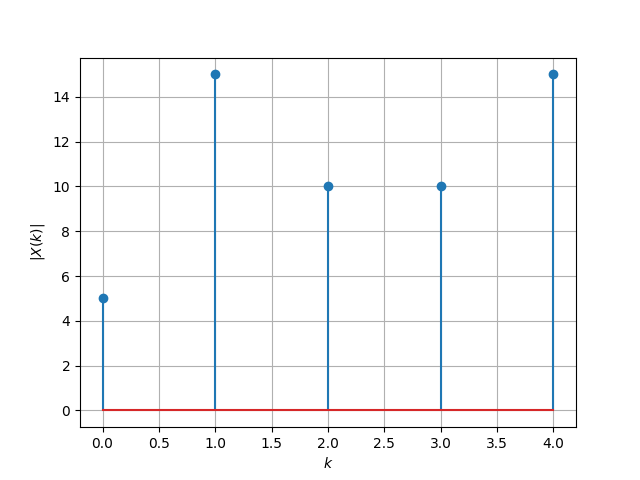
\includegraphics[width=\columnwidth]{2023/EC/47/figs/mm1.png}
    \caption{Amplitude of equation \eqref{eq:gate23ec47eq3}}
    \label{fig:gate23ec47fig1}
\end{figure}
\begin{figure}[htbp]
    \centering
    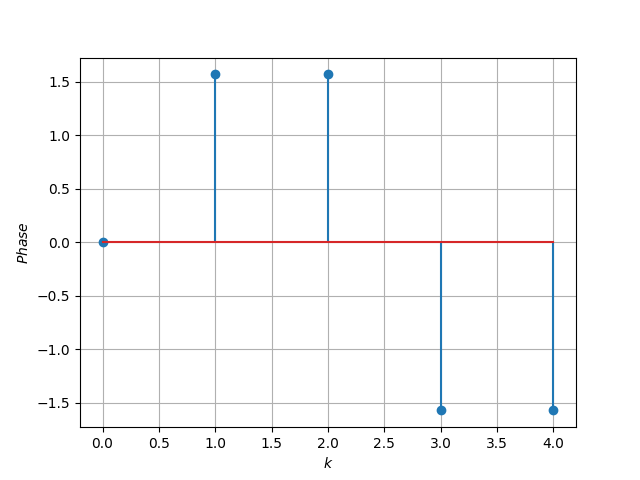
\includegraphics[width=\columnwidth]{2023/EC/47/figs/mm11.png}
    \caption{Phase of equation \eqref{eq:gate23ec47eq3}}
    \label{fig:gate23ec47fig2}
\end{figure}

\item Solving the question for N=8:
\begin{table}[h!]
 	\centering
 	\resizebox{6 cm}{!}{
 		\begin{tabular}{|c|c|c|}
    \hline
    \textbf{Parameter} & \textbf{Value} & \textbf{Description} \\[6pt]
    \hline
    $N$ &  $8$ & Time period \\ \cline{1-2}\cline{3-3}
    $X(k)$ &  $\sum\limits_{n=0}^{N-1} x(n)e^{\frac{-j2\pi kn}{N}}$ & DFT formula\\ \cline{1-2}\cline{3-3}
    $X(0)$ &  $8$ & \multirow{5}{*}{\begin{tabular}[c]{@{}c@{}}DFT \\ values\end{tabular}} \\ \cline{1-2}
    $X(1)$ &  $24j$ &    \\ \cline{1-2}
    $X(2)$ &  $16j$ &    \\ \cline{1-2}
    $X(3)$ &  $-16j$ &    \\ \cline{1-2}
    $X(4)$ &  $-24j$ &    \\ \cline{1-2}
    $X(5)$ &  $0$ &    \\ \cline{1-2}
    $X(6)$ &  $0$ &    \\ \cline{1-2}
    $X(7)$ &  $0$ &    \\ \hline
\end{tabular}

 	}
 	\vspace{6 pt}
 	\caption{Input Parameters}
 	\label{tab:gate23ec47tab1}
 \end{table} 
\begin{align}
\sum\limits_{n=0}^{7}x(n) \sin\brak{\frac{4\pi n}{8}}&=\sum\limits_{n=0}^{7}x(n)\sbrak{\frac{e^{\frac{j4\pi n}{8}}-e^{\frac{-j4\pi n}{8}}}{2j}}\\
&=\frac{1}{2j}\sbrak{\sum\limits_{n=0}^{7}x(n)e^{\frac{j2\pi (2)n}{8}}-\sum\limits_{n=0}^{7}x(n)e^{\frac{-j2\pi (2)n}{8}}}\label{eq:gate23ec47eq9}
\end{align}

Refering to the table \ref{tab:gate23ec47tab1}.
\begin{align}
X(k)&=\sum\limits_{n=0}^{7} x(n)e^{\frac{-j2\pi kn}{8}}\label{eq:gate23ec47eq10}
\end{align}
Referencing from equation\eqref{eq:gate23ec47eq10}, equation\eqref{eq:gate23ec47eq9} can be written as:
\begin{align}
\sum\limits_{n=0}^{7}x(n) \sin\brak{\frac{4\pi n}{8}}&=\frac{1}{2j}\sbrak{X(-2)-X(2)}\label{eq:gate23ec47eq11}
\end{align}
From the property of discrete Fourier series.\\
\begin{align}
X(k)=X(k+N)
\end{align}
So, equation\eqref{eq:gate23ec47eq11} becomes,\\
\begin{align}
\sum\limits_{n=0}^{7}x(n) \sin\brak{\frac{4\pi n}{8}}&=\frac{1}{2j}\sbrak{X(6)-X(2)}\\
\sum\limits_{n=0}^{7}x(n) \sin\brak{\frac{4\pi n}{8}}&=-8
\end{align}
\begin{figure}[h!]
    \centering
    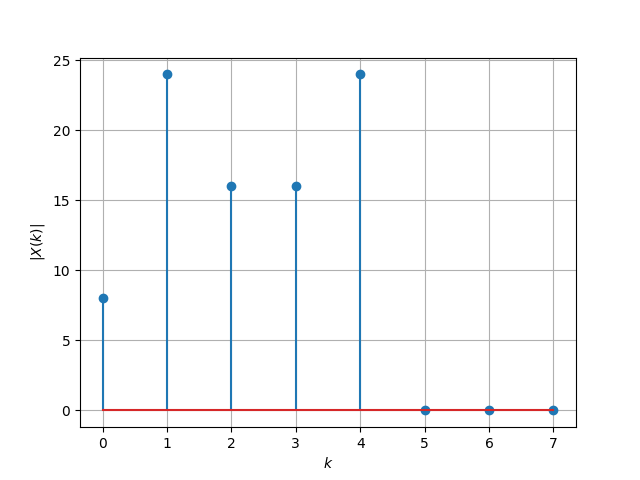
\includegraphics[width=\columnwidth]{2023/EC/47/figs/mm2.png}
    \caption{Amplitude of equation \eqref{eq:gate23ec47eq10}}
    \label{fig:gate23ec47fig3}
\end{figure}
\begin{figure}[h!]
    \centering
    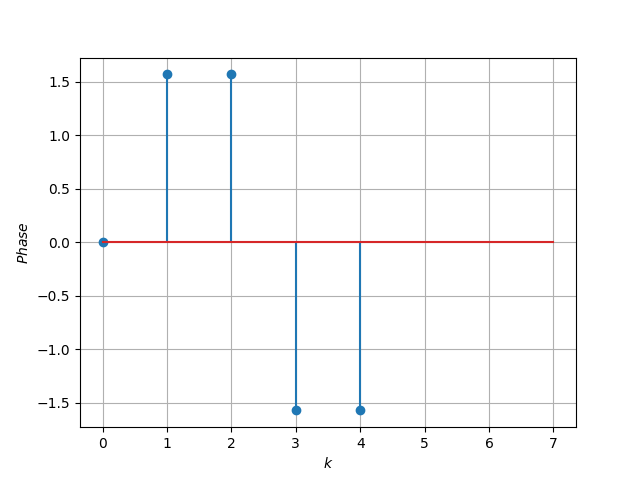
\includegraphics[width=\columnwidth]{2023/EC/47/figs/mm21.png}
    \caption{Phase of equation \eqref{eq:gate23ec47eq10}}
    \label{fig:gate23ec47fig4}
\end{figure}

\end{enumerate}

%\end{document}

\newpage
\item The figure shows a block of mass m = 20 kg attached to a pair of identical linear springs, each having a spring constant k = 1000 N/m. The block oscillates on a frictionless horizontal surface. Assuming free vibrations, the time taken by the block to complete ten oscillations is \rule{1cm}{0.15mm} seconds . (Rounded off to two decimal places) Take $\pi$ = 3.14. \\ \hfill(GATE ME 2023)

\begin{figure}[!ht]
\centering
\begin{center}
\includegraphics[width=\columnwidth]{2023/ME/30/figs/questiondiagram.jpg}
\end{center}
%\caption{Diagram for GATE ME Question 30}
\end{figure}
\solution
\input{2023/ME/30/me30.tex}
\newpage

\item A system has transfer function
 \[\frac{Y(s)}{X(s)}=\frac {s-\pi}{s+\pi}\]
 let $u(t)$ be the unit step function.The input $x(t)$ that results in a steady-state output $y(t)=sin(\pi t)$ is \underline{\quad}.\hfill (GATE IN 2023)\\
 \solution
 \iffalse
\let\negmedspace\undefined
\let\negthickspace\undefined
\documentclass[journal,12pt,twocolumn]{IEEEtran}
\usepackage{cite}
\usepackage{amsmath,amssymb,amsfonts,amsthm}
\usepackage{algorithmic}
\usepackage{graphicx}
\usepackage{textcomp}
\usepackage{xcolor}
\usepackage{txfonts}
\usepackage{listings}
\usepackage{enumitem}
\usepackage{mathtools}
\usepackage{gensymb}
\usepackage{comment}
\usepackage[breaklinks=true]{adjustbox}
\usepackage{tkz-euclide} 
\usepackage{listings}
\usepackage{gvv}                                        
\def\inputGnumericTable{}                                 
\usepackage[latin1]{inputenc}                                
\usepackage{color}                                            
\usepackage{array}                                            
\usepackage{longtable}                                       
\usepackage{calc}                                             
\usepackage{multirow}                                         
\usepackage{hhline}                                           
\usepackage{ifthen}                                           
\usepackage{lscape}

\newtheorem{theorem}{Theorem}[section]
\newtheorem{problem}{Problem}
\newtheorem{proposition}{Proposition}[section]
\newtheorem{lemma}{Lemma}[section]
\newtheorem{corollary}[theorem]{Corollary}
\newtheorem{example}{Example}[section]
\newtheorem{definition}[problem]{Definition}
\newcommand{\BEQA}{\begin{eqnarray}}
\newcommand{\EEQA}{\end{eqnarray}}
\newcommand{\define}{\stackrel{\triangle}{=}}
\theoremstyle{remark}
\newtheorem{rem}{Remark}

\begin{document}
\bibliographystyle{IEEEtran}

\vspace{3cm}

\title{}
\author{EE23BTECH11024 - G.Karthik Yadav$^{*}$
}
\maketitle
\newpage
\bigskip

\section*{GATE 2023 EC 41}
\noindent 1. \hspace{2pt} A Closed loop systen is shown in the figure where $k>0$ and $\alpha>0$ .\\
The Steady State error due to a ramp input $\brak{R\brak{s} = \alpha s^{-2}}$ is given by \hfill{(GATE 2023 EC 41)}

\begin{figure}[ht]
\centering
    \includegraphics[width=1.0\linewidth]{2023/EC/41/figs/question.png}
    \label{fig: 23.EC.41.24.1}
\end{figure}

\begin{enumerate}
\item $\frac{2\alpha}{k}$
\item $\frac{\alpha}{k}$
\item $\frac{\alpha}{2k}$
\item $\frac{\alpha}{4k}$
\end{enumerate}

\solution\\
\fi
\begin{table}[ht]
\setlength{\arrayrulewidth}{0.3mm}
\setlength{\tabcolsep}{15pt}
\renewcommand{\arraystretch}{1.5}



\begin{tabular}{ |p{1cm}|p{3cm}|p{1cm}| }
\hline
Symbol & Parameters & Value\\
\hline
$R\brak{s}$ & Laplace transform Ramp input signal r\brak{t} &  $\alpha s^{-2}$\\
\hline
$G\brak{s}$ & Open Loop transfer function &  $ \frac{Y\brak{s}}{E\brak{s}} = \frac{k}{s\brak{s+2}}$\\
\hline
$Y\brak{s}$ & Laplace transform of the output signal y\brak{t}  &  ? \\
\hline
$E\brak{s}$ & Laplace transform of the error signal e\brak{t} & R\brak{s} - Y\brak{s}\\
\hline
$E\brak{s}$ & Laplace transform of the error signal e\brak{t} & R\brak{s} - Y\brak{s}\\   
\hline
$e_s$ & Steady State Error &  ? \\
\hline
%$x(l)$ & Last($l^{th}$) term of series & 350\\
%$x(0)$ & Starting ($0^{th}$) term of series & 17 %\\
%\hline
%d & Common difference of AP & 9\\
%\hline
\end{tabular}
\caption{Parameters}






\end{table}
\bigskip
from table  Open loop transfer function $G\brak{s}$\\
\begin{align}
	G\brak{s} &= \frac{Y\brak{s}}{E\brak{s}} \label{24.2023.EC.41.1} \\
        &= \frac{Y\brak{s}}{R\brak{s} - Y\brak{s}} \\
        Y\brak{s} &= \frac{R\brak{s}G\brak{s}}{1 + G\brak{s}} \label{24.2023.EC.41.2}
\end{align}

from eq \ref{24.2023.EC.41.1} and eq \eqref{24.2023.EC.41.2}

\begin{align}
        G\brak{s} &= \frac{k}{s\brak{s +2}}  \label{24.2023.EC.41.3} \\ 
        Y\brak{s} &= \frac{\alpha k s^{-2}}{k + s\brak{s+2}} \label{24.2023.EC.41.4} \\
        E\brak{s} &= R\brak{s} - Y\brak{s}  \label{24.2023.EC.41.5} \\ 
        E\brak{s} &= \frac{\alpha \brak{s+2}}{s\brak{k + s\brak{s+2}}}
\end{align}

By Taking Inverse Laplace Transform of eq \eqref{24.2023.EC.41.3} and eq\eqref{24.2023.EC.41.4}

\begin{align}
    g\brak{t} &= \frac{k\brak{1 - e^{-2t}}}{2} u\brak{t} \\
        y\brak{t} &= \alpha t u\brak{t}- \frac{2\alpha}{k}u\brak{t} \\
        \notag &+\frac{\alpha}{2k\sqrt{1-k}} \biggl(2\sqrt{1-k}e^{\sqrt{1-k}t-1}\\ 
        \notag &+ 2\sqrt{1-k}e^{-\sqrt{1-k}t-1} \\
        \notag &+ \brak{2-k}e^{\sqrt{1-k}t-1} - \brak{2-k}e^{-\sqrt{1-k}t-1} \biggr) u\brak{t}
\end{align}

\begin{align}
        e\brak{t} &= r\brak{t} - y\brak{t} \\
        &= \alpha t u\brak{t} - y\brak{t} \\
        e\brak{t} &= \frac{2\alpha}{k}u\brak{t} \\
        \notag &-\frac{\alpha}{2k\sqrt{1-k}} \biggl(2\sqrt{1-k}e^{\sqrt{1-k}t-1}\\ 
        \notag &+ 2\sqrt{1-k}e^{-\sqrt{1-k}t-1} \\
        \notag &+ \brak{2-k}e^{\sqrt{1-k}t-1} - \brak{2-k}e^{-\sqrt{1-k}t-1} \biggr) u\brak{t}
\end{align}
	

\begin{align}
    e_s &= \displaystyle\lim_{s\to 0}s E\brak{s} \\
    &= \displaystyle\lim_{s\to 0} s \frac{R\brak{s}}{1 + G\brak{s}} \\
    &= \displaystyle\lim_{s\to 0} \frac{\alpha \brak{s+2}}{s\brak{s+2} + k} \\
    e_s &= \frac{2\alpha}{k}
\end{align}



 \newpage

\item Consider the complex function
\[ f(z) = \frac{z^{2}\sin z}{(z-\pi)^4} \]
At \( z = \pi \), which of the following options is (are) correct?
\begin{enumerate}[label=\textbf{\arabic*.}, font=\bfseries, align=left]
    \item[(A)] The order of the pole is 4 
    \item[(B)] The order of the pole is 3 
    \item[(C)] The residue at the pole is \( \frac{\pi}{6} \)
    \item[(D)] The residue at the pole is \( \frac{2\pi}{3} \)
\end{enumerate}
\hfill (GATE PH 2023)
\solution
\input{2023/PH/56/ph56.tex}
\newpage
 \item
 A buoy of virtual mass $30$ kg oscillates in a fluid medium as a single degree of
freedom system. If the total damping in the system is set as $188.5$ N-s/m, such
that the oscillation just ceases to occur, then the natural period of the system is
\rule{1cm}{0.15mm} s (round off to one decimal place)
\hfill(GATE MN 2023 question 63)\\
\solution 
\input{2023/NM/63/asnmt4.tex}
\newpage
\item 
Which of the following statement(s) is/are true?
\begin{enumerate}[label=(\alph*)]
	\item If an LTI system is causal, it is stable.
	\item A discrete time LTI system is causal if and only if its response to a step input $u[n]$ is 0 for $n < 0$.
	\item If a discrete time LTI system has an impulse response $h[n]$ of finite duration the system is stable.
	\item If the impulse response $0 < |h[n]| < 1$ for all $n$, then the LTI system is stable.
\end{enumerate}
\hfill (GATE EE 2023 question 27)\\
\solution
\iffalse
\let\negmedspace\undefined
\let\negthickspace\undefined
\documentclass[journal,12pt,twocolumn]{IEEEtran}
\usepackage{cite}
\usepackage{amsmath,amssymb,amsfonts,amsthm}
\usepackage{algorithmic}
\usepackage{graphicx}
\usepackage{textcomp}
\usepackage{xcolor}
\usepackage{txfonts}
\usepackage{listings}
\usepackage{enumitem}
\usepackage{mathtools}
\usepackage{gensymb}
\usepackage{comment}
\usepackage[breaklinks=true]{adjustbox}
\usepackage{tkz-euclide} 
\usepackage{listings}
\usepackage{gvv}                                        
\def\inputGnumericTable{}                                 
\usepackage[latin1]{inputenc}                                
\usepackage{color}                                            
\usepackage{array}                                            
\usepackage{longtable}                                       
\usepackage{calc}                                             
\usepackage{multirow}                                         
\usepackage{hhline}                                           
\usepackage{ifthen}                                           
\usepackage{lscape}

\newtheorem{theorem}{Theorem}[section]
\newtheorem{problem}{Problem}
\newtheorem{proposition}{Proposition}[section]
\newtheorem{lemma}{Lemma}[section]
\newtheorem{corollary}[theorem]{Corollary}
\newtheorem{example}{Example}[section]
\newtheorem{definition}[problem]{Definition}
\newcommand{\BEQA}{\begin{eqnarray}}
\newcommand{\EEQA}{\end{eqnarray}}
\newcommand{\define}{\stackrel{\triangle}{=}}
\theoremstyle{remark}
\newtheorem{rem}{Remark}

\begin{document}
\bibliographystyle{IEEEtran}

\vspace{3cm}

\title{}
\author{EE23BTECH11024 - G.Karthik Yadav$^{*}$
}
\maketitle
\newpage
\bigskip

\section*{GATE 2023 EC 41}
\noindent 1. \hspace{2pt} A Closed loop systen is shown in the figure where $k>0$ and $\alpha>0$ .\\
The Steady State error due to a ramp input $\brak{R\brak{s} = \alpha s^{-2}}$ is given by \hfill{(GATE 2023 EC 41)}

\begin{figure}[ht]
\centering
    \includegraphics[width=1.0\linewidth]{2023/EC/41/figs/question.png}
    \label{fig: 23.EC.41.24.1}
\end{figure}

\begin{enumerate}
\item $\frac{2\alpha}{k}$
\item $\frac{\alpha}{k}$
\item $\frac{\alpha}{2k}$
\item $\frac{\alpha}{4k}$
\end{enumerate}

\solution\\
\fi
\begin{table}[ht]
\setlength{\arrayrulewidth}{0.3mm}
\setlength{\tabcolsep}{15pt}
\renewcommand{\arraystretch}{1.5}



\begin{tabular}{ |p{1cm}|p{3cm}|p{1cm}| }
\hline
Symbol & Parameters & Value\\
\hline
$R\brak{s}$ & Laplace transform Ramp input signal r\brak{t} &  $\alpha s^{-2}$\\
\hline
$G\brak{s}$ & Open Loop transfer function &  $ \frac{Y\brak{s}}{E\brak{s}} = \frac{k}{s\brak{s+2}}$\\
\hline
$Y\brak{s}$ & Laplace transform of the output signal y\brak{t}  &  ? \\
\hline
$E\brak{s}$ & Laplace transform of the error signal e\brak{t} & R\brak{s} - Y\brak{s}\\
\hline
$E\brak{s}$ & Laplace transform of the error signal e\brak{t} & R\brak{s} - Y\brak{s}\\   
\hline
$e_s$ & Steady State Error &  ? \\
\hline
%$x(l)$ & Last($l^{th}$) term of series & 350\\
%$x(0)$ & Starting ($0^{th}$) term of series & 17 %\\
%\hline
%d & Common difference of AP & 9\\
%\hline
\end{tabular}
\caption{Parameters}






\end{table}
\bigskip
from table  Open loop transfer function $G\brak{s}$\\
\begin{align}
	G\brak{s} &= \frac{Y\brak{s}}{E\brak{s}} \label{24.2023.EC.41.1} \\
        &= \frac{Y\brak{s}}{R\brak{s} - Y\brak{s}} \\
        Y\brak{s} &= \frac{R\brak{s}G\brak{s}}{1 + G\brak{s}} \label{24.2023.EC.41.2}
\end{align}

from eq \ref{24.2023.EC.41.1} and eq \eqref{24.2023.EC.41.2}

\begin{align}
        G\brak{s} &= \frac{k}{s\brak{s +2}}  \label{24.2023.EC.41.3} \\ 
        Y\brak{s} &= \frac{\alpha k s^{-2}}{k + s\brak{s+2}} \label{24.2023.EC.41.4} \\
        E\brak{s} &= R\brak{s} - Y\brak{s}  \label{24.2023.EC.41.5} \\ 
        E\brak{s} &= \frac{\alpha \brak{s+2}}{s\brak{k + s\brak{s+2}}}
\end{align}

By Taking Inverse Laplace Transform of eq \eqref{24.2023.EC.41.3} and eq\eqref{24.2023.EC.41.4}

\begin{align}
    g\brak{t} &= \frac{k\brak{1 - e^{-2t}}}{2} u\brak{t} \\
        y\brak{t} &= \alpha t u\brak{t}- \frac{2\alpha}{k}u\brak{t} \\
        \notag &+\frac{\alpha}{2k\sqrt{1-k}} \biggl(2\sqrt{1-k}e^{\sqrt{1-k}t-1}\\ 
        \notag &+ 2\sqrt{1-k}e^{-\sqrt{1-k}t-1} \\
        \notag &+ \brak{2-k}e^{\sqrt{1-k}t-1} - \brak{2-k}e^{-\sqrt{1-k}t-1} \biggr) u\brak{t}
\end{align}

\begin{align}
        e\brak{t} &= r\brak{t} - y\brak{t} \\
        &= \alpha t u\brak{t} - y\brak{t} \\
        e\brak{t} &= \frac{2\alpha}{k}u\brak{t} \\
        \notag &-\frac{\alpha}{2k\sqrt{1-k}} \biggl(2\sqrt{1-k}e^{\sqrt{1-k}t-1}\\ 
        \notag &+ 2\sqrt{1-k}e^{-\sqrt{1-k}t-1} \\
        \notag &+ \brak{2-k}e^{\sqrt{1-k}t-1} - \brak{2-k}e^{-\sqrt{1-k}t-1} \biggr) u\brak{t}
\end{align}
	

\begin{align}
    e_s &= \displaystyle\lim_{s\to 0}s E\brak{s} \\
    &= \displaystyle\lim_{s\to 0} s \frac{R\brak{s}}{1 + G\brak{s}} \\
    &= \displaystyle\lim_{s\to 0} \frac{\alpha \brak{s+2}}{s\brak{s+2} + k} \\
    e_s &= \frac{2\alpha}{k}
\end{align}



\newpage

\item The outlet concentration $C_A$ of a plug flow reactor (PFR) is controlled by manipulating the inlet concentration $C_{A0}$.The following transfer function describes the dynamics of this PFR.
\begin{align*}
    \frac{C_{A}(s)}{C_{A0}(s)}=e^{-(\frac{V}{F})(k+s)}
\end{align*}
In the above question, V=1$m^3$,F=0.1$m^3$$min^{-1}$ and k=0.5$min^{-1}$.The measurement and valve transfer functions are both equal to 1.The ultimate gain, defined as the proportional controller gain that produces sustained oscillations, for this system is\\ \hfill{(GATE 2023 CH 61)}\\
\solution
\item For the block diagram shown in the figure, the transfer function $\frac{Y\brak{s}}{R\brak{s}}$ is \\
\begin{figure}[H]
    {\input{2023/figs/block}}
    \caption{Block diagram}
    \label{fig:gate_ee_Q12_blockdiagram}
\end{figure}
\hfill (GATE EE 2023)\\
\solution
\iffalse
\let\negmedspace\undefined
\let\negthickspace\undefined
\documentclass[journal,12pt,twocolumn]{IEEEtran}
\usepackage{cite}
\usepackage{amsmath,amssymb,amsfonts,amsthm}
\usepackage{algorithmic}
\usepackage{graphicx}
\usepackage{textcomp}
\usepackage{xcolor}
\usepackage{txfonts}
\usepackage{listings}
\usepackage{enumitem}
\usepackage{mathtools}
\usepackage{gensymb}
\usepackage{comment}
\usepackage[breaklinks=true]{adjustbox}
\usepackage{tkz-euclide} 
\usepackage{listings}
\usepackage{gvv}                                        
\def\inputGnumericTable{}                                 
\usepackage[latin1]{inputenc}                                
\usepackage{color}                                            
\usepackage{array}                                            
\usepackage{longtable}                                       
\usepackage{calc}                                             
\usepackage{multirow}                                         
\usepackage{hhline}                                           
\usepackage{ifthen}                                           
\usepackage{lscape}

\newtheorem{theorem}{Theorem}[section]
\newtheorem{problem}{Problem}
\newtheorem{proposition}{Proposition}[section]
\newtheorem{lemma}{Lemma}[section]
\newtheorem{corollary}[theorem]{Corollary}
\newtheorem{example}{Example}[section]
\newtheorem{definition}[problem]{Definition}
\newcommand{\BEQA}{\begin{eqnarray}}
\newcommand{\EEQA}{\end{eqnarray}}
\newcommand{\define}{\stackrel{\triangle}{=}}
\theoremstyle{remark}
\newtheorem{rem}{Remark}

\begin{document}
\bibliographystyle{IEEEtran}

\vspace{3cm}

\title{}
\author{EE23BTECH11024 - G.Karthik Yadav$^{*}$
}
\maketitle
\newpage
\bigskip

\section*{GATE 2023 EC 41}
\noindent 1. \hspace{2pt} A Closed loop systen is shown in the figure where $k>0$ and $\alpha>0$ .\\
The Steady State error due to a ramp input $\brak{R\brak{s} = \alpha s^{-2}}$ is given by \hfill{(GATE 2023 EC 41)}

\begin{figure}[ht]
\centering
    \includegraphics[width=1.0\linewidth]{2023/EC/41/figs/question.png}
    \label{fig: 23.EC.41.24.1}
\end{figure}

\begin{enumerate}
\item $\frac{2\alpha}{k}$
\item $\frac{\alpha}{k}$
\item $\frac{\alpha}{2k}$
\item $\frac{\alpha}{4k}$
\end{enumerate}

\solution\\
\fi
\begin{table}[ht]
\setlength{\arrayrulewidth}{0.3mm}
\setlength{\tabcolsep}{15pt}
\renewcommand{\arraystretch}{1.5}



\begin{tabular}{ |p{1cm}|p{3cm}|p{1cm}| }
\hline
Symbol & Parameters & Value\\
\hline
$R\brak{s}$ & Laplace transform Ramp input signal r\brak{t} &  $\alpha s^{-2}$\\
\hline
$G\brak{s}$ & Open Loop transfer function &  $ \frac{Y\brak{s}}{E\brak{s}} = \frac{k}{s\brak{s+2}}$\\
\hline
$Y\brak{s}$ & Laplace transform of the output signal y\brak{t}  &  ? \\
\hline
$E\brak{s}$ & Laplace transform of the error signal e\brak{t} & R\brak{s} - Y\brak{s}\\
\hline
$E\brak{s}$ & Laplace transform of the error signal e\brak{t} & R\brak{s} - Y\brak{s}\\   
\hline
$e_s$ & Steady State Error &  ? \\
\hline
%$x(l)$ & Last($l^{th}$) term of series & 350\\
%$x(0)$ & Starting ($0^{th}$) term of series & 17 %\\
%\hline
%d & Common difference of AP & 9\\
%\hline
\end{tabular}
\caption{Parameters}






\end{table}
\bigskip
from table  Open loop transfer function $G\brak{s}$\\
\begin{align}
	G\brak{s} &= \frac{Y\brak{s}}{E\brak{s}} \label{24.2023.EC.41.1} \\
        &= \frac{Y\brak{s}}{R\brak{s} - Y\brak{s}} \\
        Y\brak{s} &= \frac{R\brak{s}G\brak{s}}{1 + G\brak{s}} \label{24.2023.EC.41.2}
\end{align}

from eq \ref{24.2023.EC.41.1} and eq \eqref{24.2023.EC.41.2}

\begin{align}
        G\brak{s} &= \frac{k}{s\brak{s +2}}  \label{24.2023.EC.41.3} \\ 
        Y\brak{s} &= \frac{\alpha k s^{-2}}{k + s\brak{s+2}} \label{24.2023.EC.41.4} \\
        E\brak{s} &= R\brak{s} - Y\brak{s}  \label{24.2023.EC.41.5} \\ 
        E\brak{s} &= \frac{\alpha \brak{s+2}}{s\brak{k + s\brak{s+2}}}
\end{align}

By Taking Inverse Laplace Transform of eq \eqref{24.2023.EC.41.3} and eq\eqref{24.2023.EC.41.4}

\begin{align}
    g\brak{t} &= \frac{k\brak{1 - e^{-2t}}}{2} u\brak{t} \\
        y\brak{t} &= \alpha t u\brak{t}- \frac{2\alpha}{k}u\brak{t} \\
        \notag &+\frac{\alpha}{2k\sqrt{1-k}} \biggl(2\sqrt{1-k}e^{\sqrt{1-k}t-1}\\ 
        \notag &+ 2\sqrt{1-k}e^{-\sqrt{1-k}t-1} \\
        \notag &+ \brak{2-k}e^{\sqrt{1-k}t-1} - \brak{2-k}e^{-\sqrt{1-k}t-1} \biggr) u\brak{t}
\end{align}

\begin{align}
        e\brak{t} &= r\brak{t} - y\brak{t} \\
        &= \alpha t u\brak{t} - y\brak{t} \\
        e\brak{t} &= \frac{2\alpha}{k}u\brak{t} \\
        \notag &-\frac{\alpha}{2k\sqrt{1-k}} \biggl(2\sqrt{1-k}e^{\sqrt{1-k}t-1}\\ 
        \notag &+ 2\sqrt{1-k}e^{-\sqrt{1-k}t-1} \\
        \notag &+ \brak{2-k}e^{\sqrt{1-k}t-1} - \brak{2-k}e^{-\sqrt{1-k}t-1} \biggr) u\brak{t}
\end{align}
	

\begin{align}
    e_s &= \displaystyle\lim_{s\to 0}s E\brak{s} \\
    &= \displaystyle\lim_{s\to 0} s \frac{R\brak{s}}{1 + G\brak{s}} \\
    &= \displaystyle\lim_{s\to 0} \frac{\alpha \brak{s+2}}{s\brak{s+2} + k} \\
    e_s &= \frac{2\alpha}{k}
\end{align}



\newpage

\item In the following block diagram, $R\brak{s}$ and $D\brak{s}$ are two inputs. The output Y(s) is expressed as $Y\brak{s} = G_1\brak{s}R\brak{s} + G_2\brak{s}D\brak{s}$\\
$G_1\brak{s}$ and $G_2\brak{s}$ are given by\\
\begin{figure}[htbp!]
\centering
\iffalse
\let\negmedspace\undefined
\let\negthickspace\undefined
\documentclass[journal,12pt,twocolumn]{IEEEtran}
\usepackage{cite}
\usepackage{amsmath,amssymb,amsfonts,amsthm}
\usepackage{algorithmic}
\usepackage{graphicx}
\usepackage{textcomp}
\usepackage{xcolor}
\usepackage{txfonts}
\usepackage{listings}
\usepackage{enumitem}
\usepackage{mathtools}
\usepackage{gensymb}
\usepackage{comment}
\usepackage[breaklinks=true]{hyperref}
\usepackage{tkz-euclide} 
\usepackage{listings}
\usepackage{gvv}                                        
\def\inputGnumericTable{}                                 
\usepackage[latin1]{inputenc}                                
\usepackage{color}                                            
\usepackage{array}                                            
\usepackage{longtable}                                       
\usepackage{calc}                                             
\usepackage{multirow}                                         
\usepackage{hhline}                                           
\usepackage{ifthen}                                           
\usepackage{lscape}


\newtheorem{theorem}{Theorem}[section]
\newtheorem{problem}{Problem}
\newtheorem{proposition}{Proposition}[section]
\newtheorem{lemma}{Lemma}[section]
\newtheorem{corollary}[theorem]{Corollary}
\newtheorem{example}{Example}[section]
\newtheorem{definition}[problem]{Definition}
\newcommand{\BEQA}{\begin{eqnarray}}
\newcommand{\EEQA}{\end{eqnarray}}
\newcommand{\define}{\stackrel{\triangle}{=}}
\theoremstyle{remark}
\newtheorem{rem}{Remark}
\begin{document}
\parindent 0px
\bibliographystyle{IEEEtran}

\title{Gate EE - 18}
\author{EE23BTECH11216 - P.kalyan$^{}$% <-this % stops a space
}
\maketitle
\newpage
\bigskip

\renewcommand{\thefigure}{\theenumi}
\renewcommand{\thetable}{\theenumi}
\section*{Question}
The Fourier transform x$\brak{\omega}$ of  the signal x\brak{t} is given by

\[
X(\omega) = 
\begin{cases} 
1, \text{for } |\omega| < \omega_0 \\
0, \text{for } |\omega| > \omega_0 
\end{cases}
\]

\text{(A) } x\brak{t} \text{ tends to be an impulse as } $W_0$ $\rightarrow \infty$.

\text{(B) } x\brak{0} \text{ decreases as } $W_0$ \text{ increases.}

\text{(C) At } t = $\frac{\pi}{2W_0}$, \quad x\brak{t} = -$\frac{1}{\pi}$.

\text{(D) At } t = $\frac{\pi}{2W_0}$, \quad x\brak{t} = $\frac{1}{\pi}$. \hfill\brak{\text{GATE EE 2023}}


 \fi

\begin{center}
    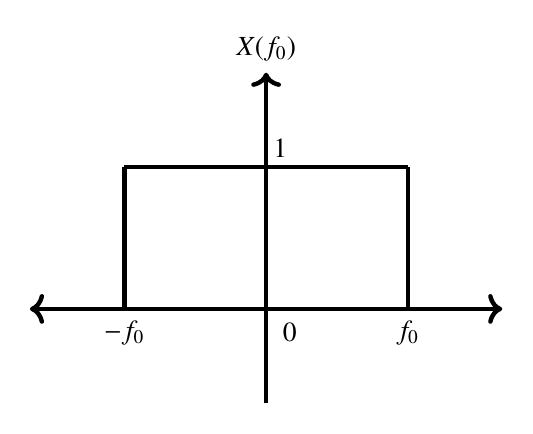
\begin{tikzpicture}[scale=0.6, ultra thick]
        \draw[->] (0,-2) -- (0,5);
        \draw (0,5.5) node {$X(f_{0}$)};
        \draw (0.5,-0.5)  node{0};
        \draw[<->]  (-5,0) -- (5,0);
        \draw  (3,3) -- (3,0);
        \draw (0.3,3.4) node{1};
        \draw (-3,3) -- (3,3);
        \draw (-3,3)--(-3,0);
        \draw (-3,-0.5) node {$-f_{0}$};

        \draw (3,-0.5) node {$f_{0}$};
    \end{tikzpicture}
\end{center}

By taking inverse Fourier transform,
\begin{align}
x\brak{t} = \frac{\sin\brak{ t}}{\pi t}
\end{align}

\begin{align}
& x\left(\frac{\pi}{2\brak{2\pi f_{0}}}\right) =\frac{2 \brak{2\pi f_{0}}}{\pi^2}
\end{align}

So, option \brak{C} and \brak{D} are wrong.

\begin{align}
x\brak{0}=\lim_{t\to 0}\frac{\sin \brak{2\pi f_{0}} t}{\pi t}=\frac{2\pi f_{0}}{\pi}
\end{align}

So, $x\brak{0} \propto f_{0} \Rightarrow$ Option \brak{B} is wrong.\\

When $f_{0}\rightarrow \infty$, $X\brak{f_{0}}$ will be a D.C signal and inverse Fourier transform of a D.C signal will be impulse signal\\[3ex]
So, option \brak{A} is correct
\begin{figure}[ht]
    \centering
    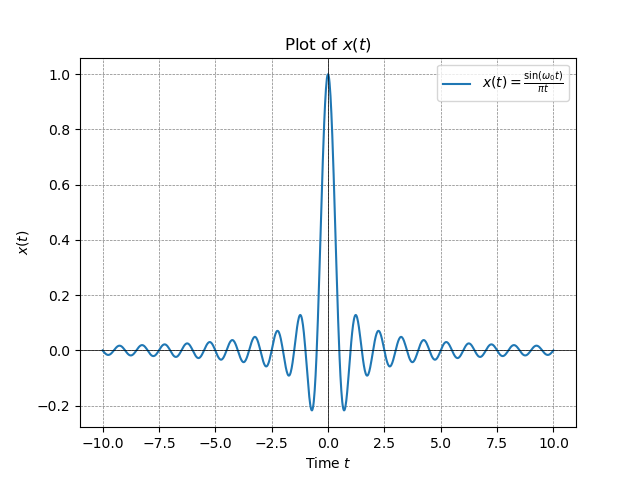
\includegraphics[width=1\columnwidth]{2023/EE/18/figs/main.png}
    \caption{plot of X\brak{t}}
    \label{fig:EE18.1}
\end{figure}


\end{figure}\\
\begin{enumerate}[label=\alph*)]
\item $G_1\brak{s} = \frac{G\brak{s}}{1+G\brak{s}+G\brak{s}H\brak{s}}$ and $G_2\brak{s} = \frac{G\brak{s}}{1+ G\brak{s}+G\brak{s}H\brak{s}}$\\
\item $G_1\brak{s} = \frac{G\brak{s}}{1+G\brak{s}+H\brak{s}}$ and $G_2\brak{s} = \frac{G\brak{s}}{1+ G\brak{s}+H\brak{s}}$\\
\item $G_1\brak{s} = \frac{G\brak{s}}{1+G\brak{s}+H\brak{s}}$ and $G_2\brak{s} = \frac{G\brak{s}}{1+ G\brak{s}+G\brak{s}H\brak{s}}$\\
\item $G_1\brak{s} = \frac{G\brak{s}}{1+G\brak{s}+G\brak{s}H\brak{s}}$ and $G_2\brak{s} = \frac{G\brak{s}}{1+ G\brak{s}+H\brak{s}}$\\
\end{enumerate}
\hfill{GATE 2023 EC Q.42}\\
\solution\\
\input{2023/EC/42/42.tex}
\newpage

\item In the table shown below, match the signal type with its spectral characteristics.\hfill{GATE 2023 EC}

\vspace{2mm}

\begin{table}[ht]
    \centering
    \def\arraystretch{2.5}
    \setlength{\arrayrulewidth}{0.3mm}
\setlength{\tabcolsep}{15pt}
\renewcommand{\arraystretch}{1.5}



\begin{tabular}{ |p{1cm}|p{3cm}|p{1cm}| }
\hline
Symbol & Parameters & Value\\
\hline
$R\brak{s}$ & Laplace transform Ramp input signal r\brak{t} &  $\alpha s^{-2}$\\
\hline
$G\brak{s}$ & Open Loop transfer function &  $ \frac{Y\brak{s}}{E\brak{s}} = \frac{k}{s\brak{s+2}}$\\
\hline
$Y\brak{s}$ & Laplace transform of the output signal y\brak{t}  &  ? \\
\hline
$E\brak{s}$ & Laplace transform of the error signal e\brak{t} & R\brak{s} - Y\brak{s}\\
\hline
$E\brak{s}$ & Laplace transform of the error signal e\brak{t} & R\brak{s} - Y\brak{s}\\   
\hline
$e_s$ & Steady State Error &  ? \\
\hline
%$x(l)$ & Last($l^{th}$) term of series & 350\\
%$x(0)$ & Starting ($0^{th}$) term of series & 17 %\\
%\hline
%d & Common difference of AP & 9\\
%\hline
\end{tabular}
\caption{Parameters}






    \caption{ }
    \label{29.2023}
\end{table}

\begin{enumerate}
\item \brak{\romannumeral 1} \textrightarrow \brak{a}  ,   \brak{\romannumeral 2} \textrightarrow \brak{b}   ,   \brak{\romannumeral 3} \textrightarrow \brak{c}   ,   \brak{\romannumeral 4} \textrightarrow \brak{d}

\item \brak{\romannumeral 1} \textrightarrow \brak{a}   ,  \brak{\romannumeral 2} \textrightarrow \brak{c}   ,   \brak{\romannumeral 3} \textrightarrow \brak{b}   ,   \brak{\romannumeral 4} \textrightarrow \brak{d}

\item  \brak{\romannumeral 1} \textrightarrow \brak{d}   ,   \brak{\romannumeral 2} \textrightarrow \brak{b}   ,   \brak{\romannumeral 3} \textrightarrow \brak{c}   ,   \brak{\romannumeral 4} \textrightarrow \brak{a}

\item \brak{\romannumeral 1} \textrightarrow \brak{a}   ,  \brak{\romannumeral 2} \textrightarrow \brak{c}    ,   \brak{\romannumeral 3} \textrightarrow \brak{d}   ,  \brak{\romannumeral 4} \textrightarrow \brak{b}

\end{enumerate}
\solution
\input{2023/EC/29/ec23.tex}
\newpage


\item
The impulse response of an LTI system is $h\brak{t}$= $\delta\brak{t}$+0.5$ \delta\brak{t-4}$, where $\delta\brak{t}$ is continuous-time unit impulse signal.If the input signal $x(t)=\cos\brak{\frac{7\pi t}{4}}$,the output is\hfill(GATE IN 2023)\\
\solution 
\iffalse
\let\negmedspace\undefined
\let\negthickspace\undefined
\documentclass[journal,12pt,twocolumn]{IEEEtran}
\usepackage{cite}
\usepackage{amsmath,amssymb,amsfonts,amsthm}
\usepackage{algorithmic}
\usepackage{graphicx}
\usepackage{textcomp}
\usepackage{xcolor}
\usepackage{txfonts}
\usepackage{listings}
\usepackage{enumitem}
\usepackage{mathtools}
\usepackage{gensymb}
\usepackage{comment}
\usepackage[breaklinks=true]{adjustbox}
\usepackage{tkz-euclide} 
\usepackage{listings}
\usepackage{gvv}                                        
\def\inputGnumericTable{}                                 
\usepackage[latin1]{inputenc}                                
\usepackage{color}                                            
\usepackage{array}                                            
\usepackage{longtable}                                       
\usepackage{calc}                                             
\usepackage{multirow}                                         
\usepackage{hhline}                                           
\usepackage{ifthen}                                           
\usepackage{lscape}

\newtheorem{theorem}{Theorem}[section]
\newtheorem{problem}{Problem}
\newtheorem{proposition}{Proposition}[section]
\newtheorem{lemma}{Lemma}[section]
\newtheorem{corollary}[theorem]{Corollary}
\newtheorem{example}{Example}[section]
\newtheorem{definition}[problem]{Definition}
\newcommand{\BEQA}{\begin{eqnarray}}
\newcommand{\EEQA}{\end{eqnarray}}
\newcommand{\define}{\stackrel{\triangle}{=}}
\theoremstyle{remark}
\newtheorem{rem}{Remark}

\begin{document}
\bibliographystyle{IEEEtran}

\vspace{3cm}

\title{}
\author{EE23BTECH11024 - G.Karthik Yadav$^{*}$
}
\maketitle
\newpage
\bigskip

\section*{GATE 2023 EC 41}
\noindent 1. \hspace{2pt} A Closed loop systen is shown in the figure where $k>0$ and $\alpha>0$ .\\
The Steady State error due to a ramp input $\brak{R\brak{s} = \alpha s^{-2}}$ is given by \hfill{(GATE 2023 EC 41)}

\begin{figure}[ht]
\centering
    \includegraphics[width=1.0\linewidth]{2023/EC/41/figs/question.png}
    \label{fig: 23.EC.41.24.1}
\end{figure}

\begin{enumerate}
\item $\frac{2\alpha}{k}$
\item $\frac{\alpha}{k}$
\item $\frac{\alpha}{2k}$
\item $\frac{\alpha}{4k}$
\end{enumerate}

\solution\\
\fi
\begin{table}[ht]
\setlength{\arrayrulewidth}{0.3mm}
\setlength{\tabcolsep}{15pt}
\renewcommand{\arraystretch}{1.5}



\begin{tabular}{ |p{1cm}|p{3cm}|p{1cm}| }
\hline
Symbol & Parameters & Value\\
\hline
$R\brak{s}$ & Laplace transform Ramp input signal r\brak{t} &  $\alpha s^{-2}$\\
\hline
$G\brak{s}$ & Open Loop transfer function &  $ \frac{Y\brak{s}}{E\brak{s}} = \frac{k}{s\brak{s+2}}$\\
\hline
$Y\brak{s}$ & Laplace transform of the output signal y\brak{t}  &  ? \\
\hline
$E\brak{s}$ & Laplace transform of the error signal e\brak{t} & R\brak{s} - Y\brak{s}\\
\hline
$E\brak{s}$ & Laplace transform of the error signal e\brak{t} & R\brak{s} - Y\brak{s}\\   
\hline
$e_s$ & Steady State Error &  ? \\
\hline
%$x(l)$ & Last($l^{th}$) term of series & 350\\
%$x(0)$ & Starting ($0^{th}$) term of series & 17 %\\
%\hline
%d & Common difference of AP & 9\\
%\hline
\end{tabular}
\caption{Parameters}






\end{table}
\bigskip
from table  Open loop transfer function $G\brak{s}$\\
\begin{align}
	G\brak{s} &= \frac{Y\brak{s}}{E\brak{s}} \label{24.2023.EC.41.1} \\
        &= \frac{Y\brak{s}}{R\brak{s} - Y\brak{s}} \\
        Y\brak{s} &= \frac{R\brak{s}G\brak{s}}{1 + G\brak{s}} \label{24.2023.EC.41.2}
\end{align}

from eq \ref{24.2023.EC.41.1} and eq \eqref{24.2023.EC.41.2}

\begin{align}
        G\brak{s} &= \frac{k}{s\brak{s +2}}  \label{24.2023.EC.41.3} \\ 
        Y\brak{s} &= \frac{\alpha k s^{-2}}{k + s\brak{s+2}} \label{24.2023.EC.41.4} \\
        E\brak{s} &= R\brak{s} - Y\brak{s}  \label{24.2023.EC.41.5} \\ 
        E\brak{s} &= \frac{\alpha \brak{s+2}}{s\brak{k + s\brak{s+2}}}
\end{align}

By Taking Inverse Laplace Transform of eq \eqref{24.2023.EC.41.3} and eq\eqref{24.2023.EC.41.4}

\begin{align}
    g\brak{t} &= \frac{k\brak{1 - e^{-2t}}}{2} u\brak{t} \\
        y\brak{t} &= \alpha t u\brak{t}- \frac{2\alpha}{k}u\brak{t} \\
        \notag &+\frac{\alpha}{2k\sqrt{1-k}} \biggl(2\sqrt{1-k}e^{\sqrt{1-k}t-1}\\ 
        \notag &+ 2\sqrt{1-k}e^{-\sqrt{1-k}t-1} \\
        \notag &+ \brak{2-k}e^{\sqrt{1-k}t-1} - \brak{2-k}e^{-\sqrt{1-k}t-1} \biggr) u\brak{t}
\end{align}

\begin{align}
        e\brak{t} &= r\brak{t} - y\brak{t} \\
        &= \alpha t u\brak{t} - y\brak{t} \\
        e\brak{t} &= \frac{2\alpha}{k}u\brak{t} \\
        \notag &-\frac{\alpha}{2k\sqrt{1-k}} \biggl(2\sqrt{1-k}e^{\sqrt{1-k}t-1}\\ 
        \notag &+ 2\sqrt{1-k}e^{-\sqrt{1-k}t-1} \\
        \notag &+ \brak{2-k}e^{\sqrt{1-k}t-1} - \brak{2-k}e^{-\sqrt{1-k}t-1} \biggr) u\brak{t}
\end{align}
	

\begin{align}
    e_s &= \displaystyle\lim_{s\to 0}s E\brak{s} \\
    &= \displaystyle\lim_{s\to 0} s \frac{R\brak{s}}{1 + G\brak{s}} \\
    &= \displaystyle\lim_{s\to 0} \frac{\alpha \brak{s+2}}{s\brak{s+2} + k} \\
    e_s &= \frac{2\alpha}{k}
\end{align}



\newpage

\newpage

\item Consider the state-space description of an LTI system with matrices
\[ 
A = \begin{bmatrix} 0 & 1 \\ -1 & -2 \end{bmatrix}, \quad 
B = \begin{bmatrix} 0 \\ 1 \end{bmatrix}, \quad 
C = \begin{bmatrix} 3 & -2 \end{bmatrix}, \quad 
D = 1 
\]

For the input, $\sin(\omega t)$, $\omega > 0$, the value of $\omega$ for which the steady-state output of the system will be zero, is \underline{\hspace{2cm}} (Round off to the nearest integer).
\hfill(GATE 2023 EE Q46)\\
\solution
\input{2023/EE/46/gate46.tex}
\newpage

\item A causal, discrete time system is described by the difference equation $y[n] = 0.5 y[n-1] + x[n]$, for all $n$, where $y[n]$ denotes the output sequence and $x[n]$ denotes the input sequence. Which of the following statements is/are TRUE?

\begin{enumerate}[label = (\alph*)]
	\item he system has an impulse response described by $0.5^{n} u[-n]$ where $u[n]$ is the  
unit step sequence. 		
	\item The system is stable in the bounded input, bounded output sense.
	\item The system has an infinite number of non-zero samples in its impulse response
	\item The system has a finite number of non-zero samples in its impulse response.
\end{enumerate}

\hfill(GATE 2023 BM-26)\\
\solution
\iffalse
\let\negmedspace\undefined
\let\negthickspace\undefined
\documentclass[journal,12pt,twocolumn]{IEEEtran}
\usepackage{cite}
\usepackage{amsmath,amssymb,amsfonts,amsthm}
\usepackage{algorithmic}
\usepackage{graphicx}
\usepackage{textcomp}
\usepackage{xcolor}
\usepackage{txfonts}
\usepackage{listings}
\usepackage{enumitem}
\usepackage{mathtools}
\usepackage{gensymb}
\usepackage{comment}
\usepackage[breaklinks=true]{adjustbox}
\usepackage{tkz-euclide} 
\usepackage{listings}
\usepackage{gvv}                                        
\def\inputGnumericTable{}                                 
\usepackage[latin1]{inputenc}                                
\usepackage{color}                                            
\usepackage{array}                                            
\usepackage{longtable}                                       
\usepackage{calc}                                             
\usepackage{multirow}                                         
\usepackage{hhline}                                           
\usepackage{ifthen}                                           
\usepackage{lscape}

\newtheorem{theorem}{Theorem}[section]
\newtheorem{problem}{Problem}
\newtheorem{proposition}{Proposition}[section]
\newtheorem{lemma}{Lemma}[section]
\newtheorem{corollary}[theorem]{Corollary}
\newtheorem{example}{Example}[section]
\newtheorem{definition}[problem]{Definition}
\newcommand{\BEQA}{\begin{eqnarray}}
\newcommand{\EEQA}{\end{eqnarray}}
\newcommand{\define}{\stackrel{\triangle}{=}}
\theoremstyle{remark}
\newtheorem{rem}{Remark}

\begin{document}
\bibliographystyle{IEEEtran}

\vspace{3cm}

\title{}
\author{EE23BTECH11024 - G.Karthik Yadav$^{*}$
}
\maketitle
\newpage
\bigskip

\section*{GATE 2023 EC 41}
\noindent 1. \hspace{2pt} A Closed loop systen is shown in the figure where $k>0$ and $\alpha>0$ .\\
The Steady State error due to a ramp input $\brak{R\brak{s} = \alpha s^{-2}}$ is given by \hfill{(GATE 2023 EC 41)}

\begin{figure}[ht]
\centering
    \includegraphics[width=1.0\linewidth]{2023/EC/41/figs/question.png}
    \label{fig: 23.EC.41.24.1}
\end{figure}

\begin{enumerate}
\item $\frac{2\alpha}{k}$
\item $\frac{\alpha}{k}$
\item $\frac{\alpha}{2k}$
\item $\frac{\alpha}{4k}$
\end{enumerate}

\solution\\
\fi
\begin{table}[ht]
\setlength{\arrayrulewidth}{0.3mm}
\setlength{\tabcolsep}{15pt}
\renewcommand{\arraystretch}{1.5}



\begin{tabular}{ |p{1cm}|p{3cm}|p{1cm}| }
\hline
Symbol & Parameters & Value\\
\hline
$R\brak{s}$ & Laplace transform Ramp input signal r\brak{t} &  $\alpha s^{-2}$\\
\hline
$G\brak{s}$ & Open Loop transfer function &  $ \frac{Y\brak{s}}{E\brak{s}} = \frac{k}{s\brak{s+2}}$\\
\hline
$Y\brak{s}$ & Laplace transform of the output signal y\brak{t}  &  ? \\
\hline
$E\brak{s}$ & Laplace transform of the error signal e\brak{t} & R\brak{s} - Y\brak{s}\\
\hline
$E\brak{s}$ & Laplace transform of the error signal e\brak{t} & R\brak{s} - Y\brak{s}\\   
\hline
$e_s$ & Steady State Error &  ? \\
\hline
%$x(l)$ & Last($l^{th}$) term of series & 350\\
%$x(0)$ & Starting ($0^{th}$) term of series & 17 %\\
%\hline
%d & Common difference of AP & 9\\
%\hline
\end{tabular}
\caption{Parameters}






\end{table}
\bigskip
from table  Open loop transfer function $G\brak{s}$\\
\begin{align}
	G\brak{s} &= \frac{Y\brak{s}}{E\brak{s}} \label{24.2023.EC.41.1} \\
        &= \frac{Y\brak{s}}{R\brak{s} - Y\brak{s}} \\
        Y\brak{s} &= \frac{R\brak{s}G\brak{s}}{1 + G\brak{s}} \label{24.2023.EC.41.2}
\end{align}

from eq \ref{24.2023.EC.41.1} and eq \eqref{24.2023.EC.41.2}

\begin{align}
        G\brak{s} &= \frac{k}{s\brak{s +2}}  \label{24.2023.EC.41.3} \\ 
        Y\brak{s} &= \frac{\alpha k s^{-2}}{k + s\brak{s+2}} \label{24.2023.EC.41.4} \\
        E\brak{s} &= R\brak{s} - Y\brak{s}  \label{24.2023.EC.41.5} \\ 
        E\brak{s} &= \frac{\alpha \brak{s+2}}{s\brak{k + s\brak{s+2}}}
\end{align}

By Taking Inverse Laplace Transform of eq \eqref{24.2023.EC.41.3} and eq\eqref{24.2023.EC.41.4}

\begin{align}
    g\brak{t} &= \frac{k\brak{1 - e^{-2t}}}{2} u\brak{t} \\
        y\brak{t} &= \alpha t u\brak{t}- \frac{2\alpha}{k}u\brak{t} \\
        \notag &+\frac{\alpha}{2k\sqrt{1-k}} \biggl(2\sqrt{1-k}e^{\sqrt{1-k}t-1}\\ 
        \notag &+ 2\sqrt{1-k}e^{-\sqrt{1-k}t-1} \\
        \notag &+ \brak{2-k}e^{\sqrt{1-k}t-1} - \brak{2-k}e^{-\sqrt{1-k}t-1} \biggr) u\brak{t}
\end{align}

\begin{align}
        e\brak{t} &= r\brak{t} - y\brak{t} \\
        &= \alpha t u\brak{t} - y\brak{t} \\
        e\brak{t} &= \frac{2\alpha}{k}u\brak{t} \\
        \notag &-\frac{\alpha}{2k\sqrt{1-k}} \biggl(2\sqrt{1-k}e^{\sqrt{1-k}t-1}\\ 
        \notag &+ 2\sqrt{1-k}e^{-\sqrt{1-k}t-1} \\
        \notag &+ \brak{2-k}e^{\sqrt{1-k}t-1} - \brak{2-k}e^{-\sqrt{1-k}t-1} \biggr) u\brak{t}
\end{align}
	

\begin{align}
    e_s &= \displaystyle\lim_{s\to 0}s E\brak{s} \\
    &= \displaystyle\lim_{s\to 0} s \frac{R\brak{s}}{1 + G\brak{s}} \\
    &= \displaystyle\lim_{s\to 0} \frac{\alpha \brak{s+2}}{s\brak{s+2} + k} \\
    e_s &= \frac{2\alpha}{k}
\end{align}



\newpage

\item A closed loop system is shown in the figure where $k>0$ and $\alpha>0$. The steady state
error due to a ramp input $\brak{R\brak{s} = \alpha s^{-2}}$  is given by \hfill{(GATE 2023 EC 41)}

\begin{figure}[ht]
\centering
    \includegraphics[width=1.0\linewidth]{2023/EC/41/figs/question.png}
\end{figure}
\begin{enumerate}[label = (\alph*)]
  \item $\frac{2\alpha}{k}$    
  \item $\frac{\alpha}{k}$
  \item $\frac{\alpha}{2k}$
  \item $\frac{\alpha}{4k}$
\end{enumerate}
    
\solution
\iffalse
\let\negmedspace\undefined
\let\negthickspace\undefined
\documentclass[journal,12pt,twocolumn]{IEEEtran}
\usepackage{cite}
\usepackage{amsmath,amssymb,amsfonts,amsthm}
\usepackage{algorithmic}
\usepackage{graphicx}
\usepackage{textcomp}
\usepackage{xcolor}
\usepackage{txfonts}
\usepackage{listings}
\usepackage{enumitem}
\usepackage{mathtools}
\usepackage{gensymb}
\usepackage{comment}
\usepackage[breaklinks=true]{adjustbox}
\usepackage{tkz-euclide} 
\usepackage{listings}
\usepackage{gvv}                                        
\def\inputGnumericTable{}                                 
\usepackage[latin1]{inputenc}                                
\usepackage{color}                                            
\usepackage{array}                                            
\usepackage{longtable}                                       
\usepackage{calc}                                             
\usepackage{multirow}                                         
\usepackage{hhline}                                           
\usepackage{ifthen}                                           
\usepackage{lscape}

\newtheorem{theorem}{Theorem}[section]
\newtheorem{problem}{Problem}
\newtheorem{proposition}{Proposition}[section]
\newtheorem{lemma}{Lemma}[section]
\newtheorem{corollary}[theorem]{Corollary}
\newtheorem{example}{Example}[section]
\newtheorem{definition}[problem]{Definition}
\newcommand{\BEQA}{\begin{eqnarray}}
\newcommand{\EEQA}{\end{eqnarray}}
\newcommand{\define}{\stackrel{\triangle}{=}}
\theoremstyle{remark}
\newtheorem{rem}{Remark}

\begin{document}
\bibliographystyle{IEEEtran}

\vspace{3cm}

\title{}
\author{EE23BTECH11024 - G.Karthik Yadav$^{*}$
}
\maketitle
\newpage
\bigskip

\section*{GATE 2023 EC 41}
\noindent 1. \hspace{2pt} A Closed loop systen is shown in the figure where $k>0$ and $\alpha>0$ .\\
The Steady State error due to a ramp input $\brak{R\brak{s} = \alpha s^{-2}}$ is given by \hfill{(GATE 2023 EC 41)}

\begin{figure}[ht]
\centering
    \includegraphics[width=1.0\linewidth]{2023/EC/41/figs/question.png}
    \label{fig: 23.EC.41.24.1}
\end{figure}

\begin{enumerate}
\item $\frac{2\alpha}{k}$
\item $\frac{\alpha}{k}$
\item $\frac{\alpha}{2k}$
\item $\frac{\alpha}{4k}$
\end{enumerate}

\solution\\
\fi
\begin{table}[ht]
\setlength{\arrayrulewidth}{0.3mm}
\setlength{\tabcolsep}{15pt}
\renewcommand{\arraystretch}{1.5}



\begin{tabular}{ |p{1cm}|p{3cm}|p{1cm}| }
\hline
Symbol & Parameters & Value\\
\hline
$R\brak{s}$ & Laplace transform Ramp input signal r\brak{t} &  $\alpha s^{-2}$\\
\hline
$G\brak{s}$ & Open Loop transfer function &  $ \frac{Y\brak{s}}{E\brak{s}} = \frac{k}{s\brak{s+2}}$\\
\hline
$Y\brak{s}$ & Laplace transform of the output signal y\brak{t}  &  ? \\
\hline
$E\brak{s}$ & Laplace transform of the error signal e\brak{t} & R\brak{s} - Y\brak{s}\\
\hline
$E\brak{s}$ & Laplace transform of the error signal e\brak{t} & R\brak{s} - Y\brak{s}\\   
\hline
$e_s$ & Steady State Error &  ? \\
\hline
%$x(l)$ & Last($l^{th}$) term of series & 350\\
%$x(0)$ & Starting ($0^{th}$) term of series & 17 %\\
%\hline
%d & Common difference of AP & 9\\
%\hline
\end{tabular}
\caption{Parameters}






\end{table}
\bigskip
from table  Open loop transfer function $G\brak{s}$\\
\begin{align}
	G\brak{s} &= \frac{Y\brak{s}}{E\brak{s}} \label{24.2023.EC.41.1} \\
        &= \frac{Y\brak{s}}{R\brak{s} - Y\brak{s}} \\
        Y\brak{s} &= \frac{R\brak{s}G\brak{s}}{1 + G\brak{s}} \label{24.2023.EC.41.2}
\end{align}

from eq \ref{24.2023.EC.41.1} and eq \eqref{24.2023.EC.41.2}

\begin{align}
        G\brak{s} &= \frac{k}{s\brak{s +2}}  \label{24.2023.EC.41.3} \\ 
        Y\brak{s} &= \frac{\alpha k s^{-2}}{k + s\brak{s+2}} \label{24.2023.EC.41.4} \\
        E\brak{s} &= R\brak{s} - Y\brak{s}  \label{24.2023.EC.41.5} \\ 
        E\brak{s} &= \frac{\alpha \brak{s+2}}{s\brak{k + s\brak{s+2}}}
\end{align}

By Taking Inverse Laplace Transform of eq \eqref{24.2023.EC.41.3} and eq\eqref{24.2023.EC.41.4}

\begin{align}
    g\brak{t} &= \frac{k\brak{1 - e^{-2t}}}{2} u\brak{t} \\
        y\brak{t} &= \alpha t u\brak{t}- \frac{2\alpha}{k}u\brak{t} \\
        \notag &+\frac{\alpha}{2k\sqrt{1-k}} \biggl(2\sqrt{1-k}e^{\sqrt{1-k}t-1}\\ 
        \notag &+ 2\sqrt{1-k}e^{-\sqrt{1-k}t-1} \\
        \notag &+ \brak{2-k}e^{\sqrt{1-k}t-1} - \brak{2-k}e^{-\sqrt{1-k}t-1} \biggr) u\brak{t}
\end{align}

\begin{align}
        e\brak{t} &= r\brak{t} - y\brak{t} \\
        &= \alpha t u\brak{t} - y\brak{t} \\
        e\brak{t} &= \frac{2\alpha}{k}u\brak{t} \\
        \notag &-\frac{\alpha}{2k\sqrt{1-k}} \biggl(2\sqrt{1-k}e^{\sqrt{1-k}t-1}\\ 
        \notag &+ 2\sqrt{1-k}e^{-\sqrt{1-k}t-1} \\
        \notag &+ \brak{2-k}e^{\sqrt{1-k}t-1} - \brak{2-k}e^{-\sqrt{1-k}t-1} \biggr) u\brak{t}
\end{align}
	

\begin{align}
    e_s &= \displaystyle\lim_{s\to 0}s E\brak{s} \\
    &= \displaystyle\lim_{s\to 0} s \frac{R\brak{s}}{1 + G\brak{s}} \\
    &= \displaystyle\lim_{s\to 0} \frac{\alpha \brak{s+2}}{s\brak{s+2} + k} \\
    e_s &= \frac{2\alpha}{k}
\end{align}



\newpage

\end{enumerate}
